\documentclass[12pt,a4paper]{article}
\synctex=1
\usepackage[utf8]{inputenc}
\usepackage[margin=1cm]{geometry}
\usepackage{graphicx}
%\usepackage{verbatim}
\usepackage{listings}
\usepackage{multicol}
\usepackage{libertine}
\usepackage{pgfornament}
\usepackage{eso-pic}
\usepackage{textcomp}
\usepackage{courier}
\usepackage[hangul]{kotex}
\linespread{1.3}

\title{
	\centering
	\pgfornament[width=12cm,color=teal]{84}\\
	\vspace{1cm}
	\fontsize{50}{50} \selectfont {시스템 S/W 실습5}\\
	\pgfornament[width=12cm,color=teal]{88}\\
	\vfill}
\author{
	\LARGE
	\begin{tabular}{rl}
		\hline
		학번 : & 2016110056\\ 
		학과 : & 불교학부 \\
		이름 : & 박승원\\
		날짜 : & \today\\
		\hline
	\end{tabular}\vspace{2cm}
	\\
	\includegraphics[width=0.5\textwidth]{/home/zezeon/Dropbox/Photos/logo.jpg}
}
\date{}

\begin{document}
\maketitle
\noindent
\lstset{columns=flexible, tabsize=4, frame=single, showstringspaces=false, breaklines=true, upquote=true}
\begin{enumerate}

\pagenumbering{gobble}
\lstset{language=C}
%\begin{multicols}{2}
\item 다음에 주어진 프로그램 참고해서, srcfile(입력파일)을 읽고 각 줄(line)을 LABEL, OPCODE, OPERAND로 분리해서 intfile(임시출력파일)에 저장하는 프로그램을 작성해서 test5.c로 저장하고, test5.c를 Compile 하여 test run하시오. \\
단 C Program compile 명령은 다음과 같고, test의 입력파일 srcfile(SIC 어셈블리어 프로그램 파일)은 각자 준비한다.

\$gcc -0 test5 test5.c\\
\$./test5 srcfile intfile

\lstinputlisting[title=test5.c]{test4.c}

\lstinputlisting[title=srcfile]{1.s}
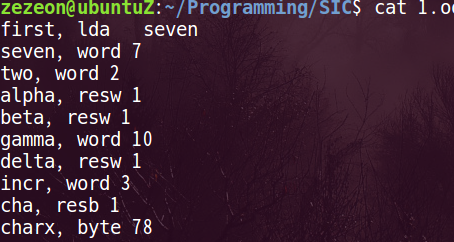
\includegraphics[width=0.7\textwidth]{test5.png}

\item 1의 내용을 확장하여 기호표 SYMTAB[]을 생성하는 프로그램을 작성하고  test하시오.

이미 지난 번에 낸 리포트에서 symtab을 컴파일러를 구현한 부분은 제출했으므로, 이번 시간에 배운 링크 부분을 매우 조악하게나마 구현한 것을 올립니다.
현재 구현한 링커에서는 다음과 같은 제한 사항이 존재합니다.
\begin{itemize}
	\item 목적파일의 이름이 반드시 숫자.o의 형식이어야 한다.
	\item 프로그램 시작 번지가 위의 파일의 숫자보다 커야 한다.
	\item 한 파일에서 서브루틴을 부를 때에 위의 숫자를 오퍼란드로 해야 한다.
	\item 링커의 명령어 라인 변수 중 첫번째가 메인 함수 진입점이 된다.
\end{itemize}
지난 시간까지 기존에 만들어 둔 소스를 최대한 적게 고치기 위해 임기응변으로 한 것입니다.
학습용으로 구현한 것이기에 사용자 편의성은 크게 신경쓰지 못함을 이해해 주시기 바랍니다.

\lstinputlisting[title=헤더파일]{link.h}
\lstinputlisting[title=구현부]{link.cc}
\lstinputlisting[title=실행화일]{linker.cpp}

링커를 테스트 하기 위한 소스파일. jsub 2 이 부분이 2.o 서브루틴을 부른다.
\lstinputlisting[title=소스파일 1.s]{1.s}
\lstinputlisting[title=목적파일 1.o]{1.o}

서브루틴이 되는 파일. 현재로서는 실제로 서브루틴의 역할을 하는 소스가 아니라 그냥 메모리에 링크해서 올리기 위한 소스입니다.
\lstinputlisting[title=소스파일 2.s]{2.s}
\lstinputlisting[title=목적파일 2.o]{2.o}

linker.x 1 2 를 실행한 결과물인 링크된 파일
\lstinputlisting[title=1.o와 2.o를 입력받아 출력된 링크된 파일]{1.x}
두번째 목적파일이 첫번째 목적파일의 위에 0x1039부터 이어져 있고, 오퍼란드의 주소가 모두 오프셋에 맞게 변경되어 있다. 
또한, 0x101e번지에서 서브루틴을 부르는 부분이 이 시작지점인 0x1039로 제대로 위치를 찾아주고 있다.
\end{enumerate}

{\Huge소감}
\indent
이상하게도 실습의 진도와 수업의 진도가 묘하게 엇박자가 난다. 수업시간에 배운 것을 그 다음 실습 시간에 하는 것이 정상이고, 학생들의 실력향상에도 도움이 되지 않을까 하고 생각한다.
\end{document}
